\documentclass[index]{subfiles}

\begin{document}
  \chapter{ゲームの紹介}
  \label{ch:first}

  Programming Partyは、カードを使って決められた仕様に従い、全員でプログラミングを行うゲームです。
  
  \begin{center}
    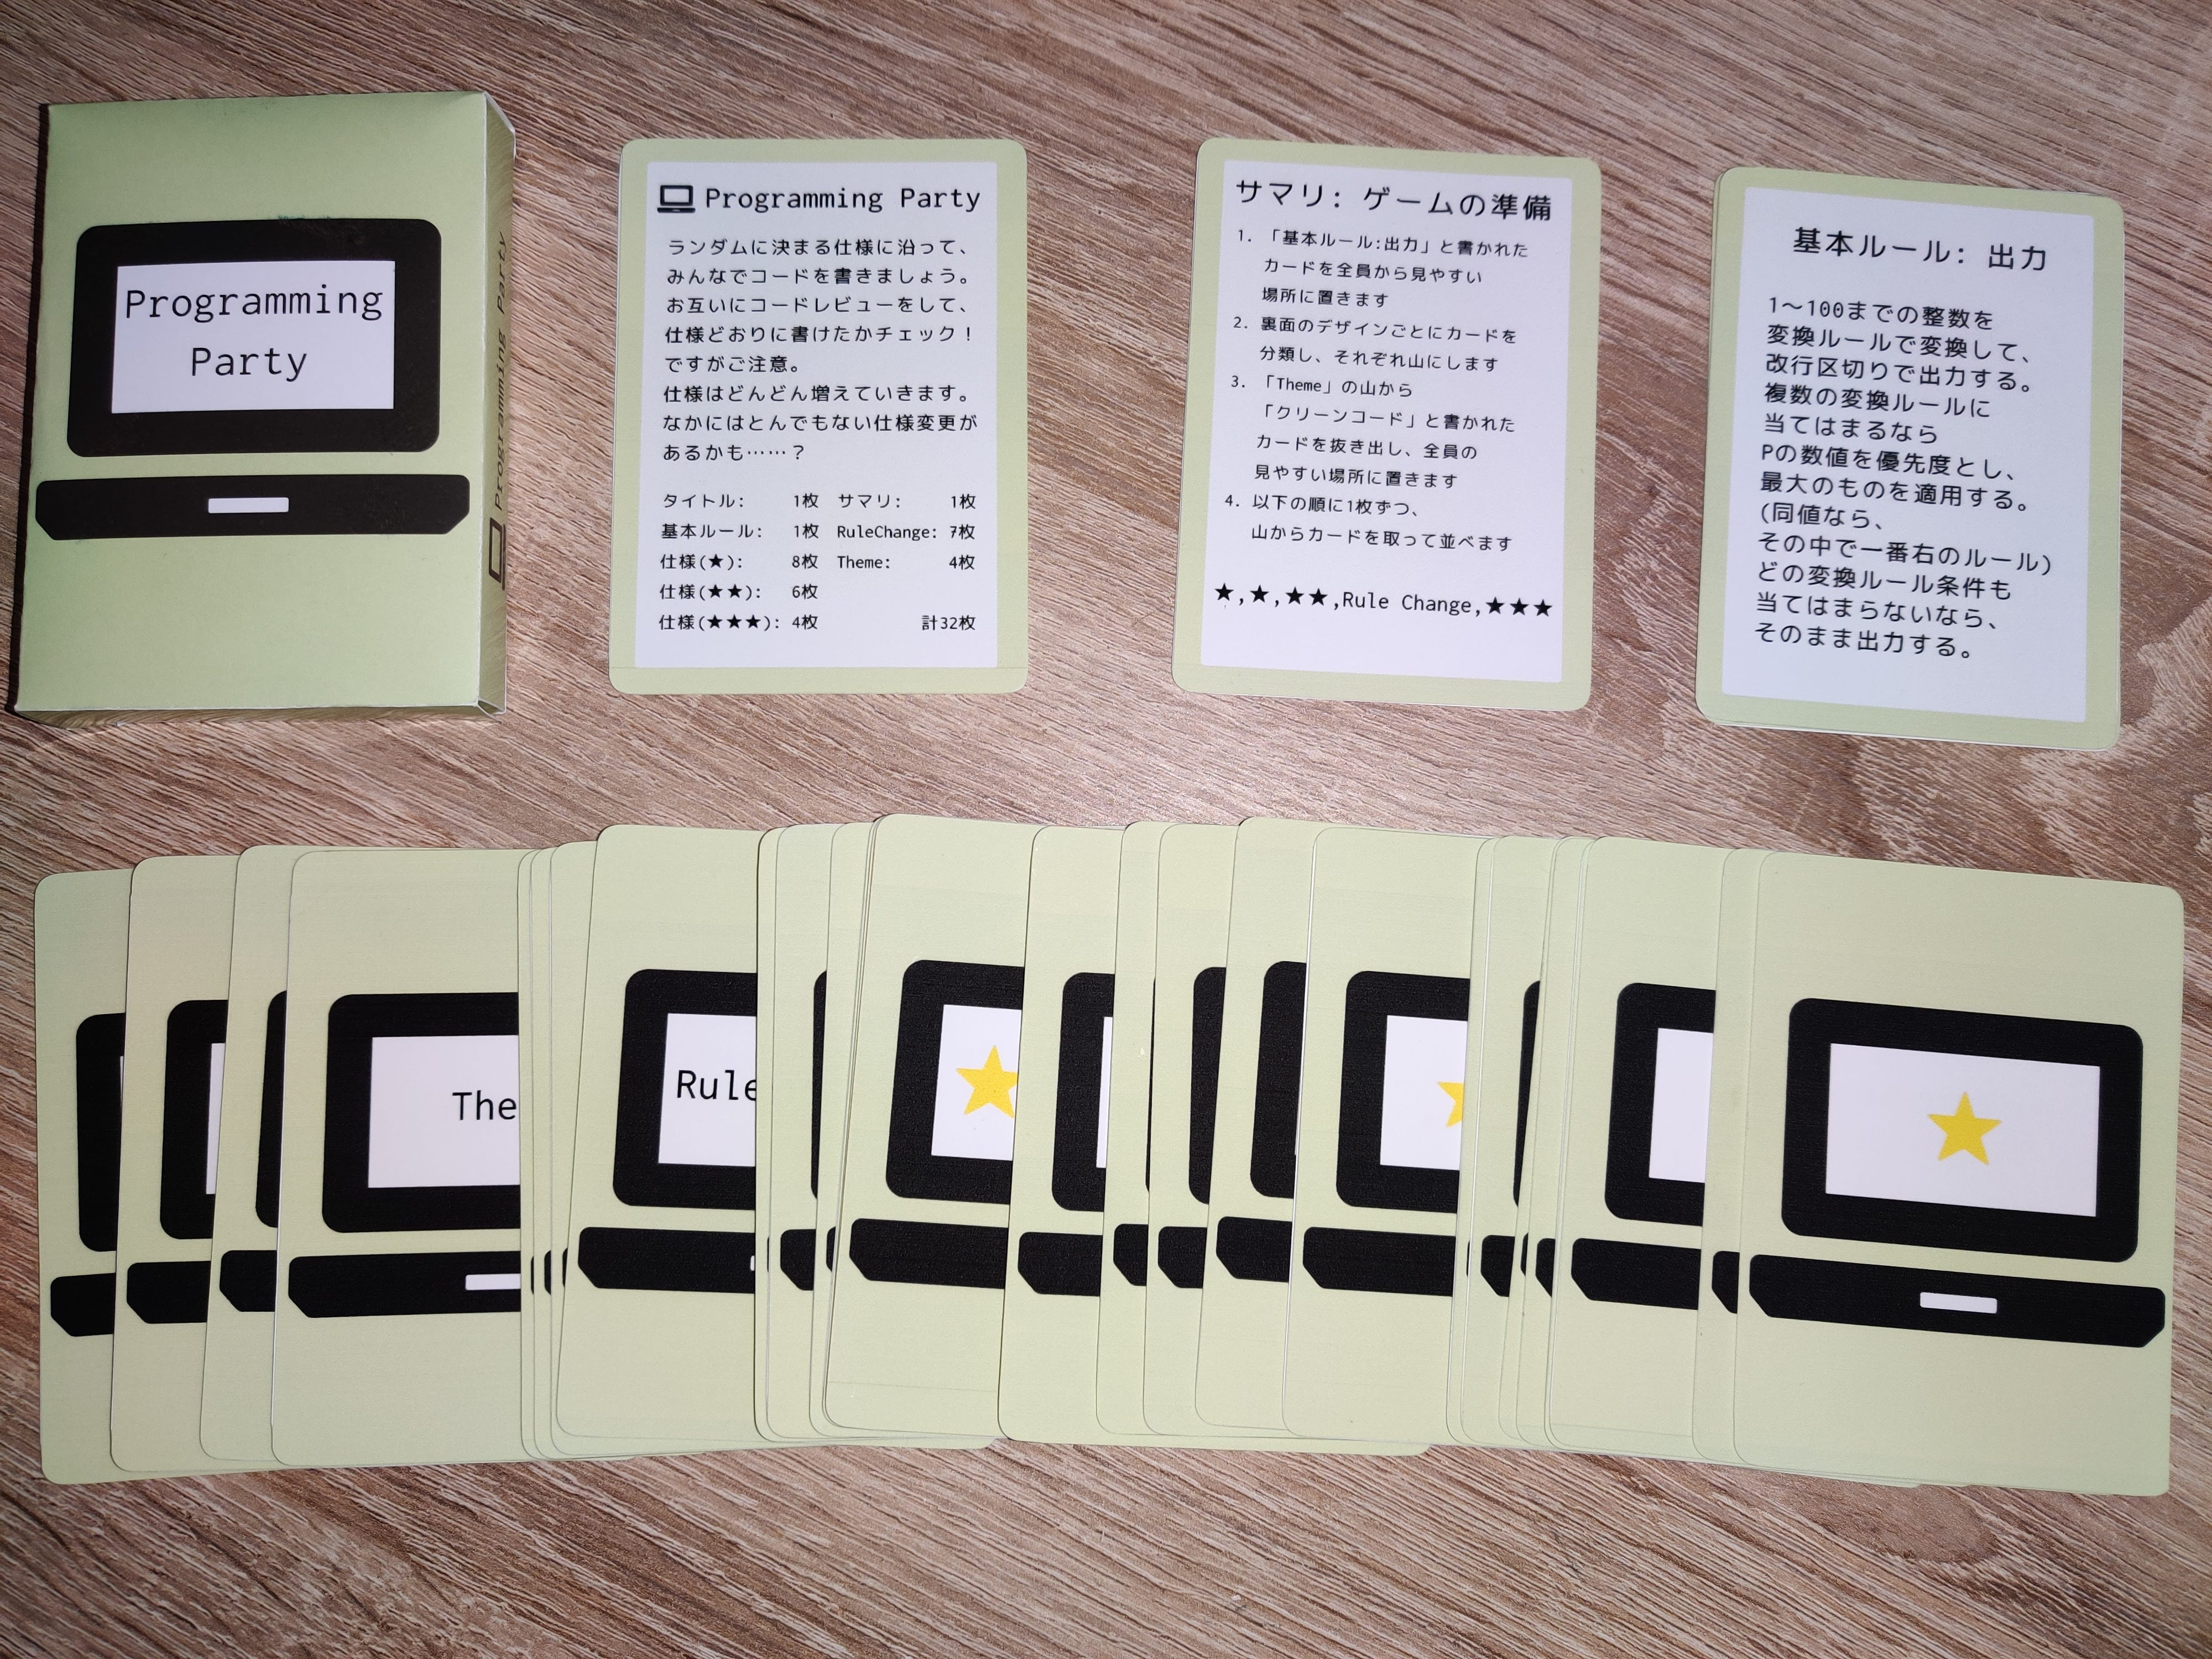
\includegraphics[height=5cm]{image/100_game_cards.jpg}
  \end{center}

  この章では、Programming Partyのコンポーネントやルールについて解説します。なお、本章の内容はオンラインマニュアル \footnote{ \url{ https://www.kokuyouwind.com/programming_party }} とほぼ同じものになっています。オンラインマニュアルは最新の修正を反映しており、FAQやエラッタもそちらに掲載いたしますので、プレイの際はそちらもご覧ください。

  \section{カードの種類}
  \label{sec:game_cardtype}

  Programming Partyはいくつかの種類のカードを用いてゲームを行います。カードはゲーム上使用しないものを除くと、以下のように分けられます。
  
  \begin{itemize}
  \item 基本ルールカード
  \item 仕様カード
  \item Rule Changeカード
  \item Themeカード
  \end{itemize}

 これらのカードは、それぞれ裏面が異なるデザインになっています。

  \subsection{基本ルールカード}

\begin{center}
  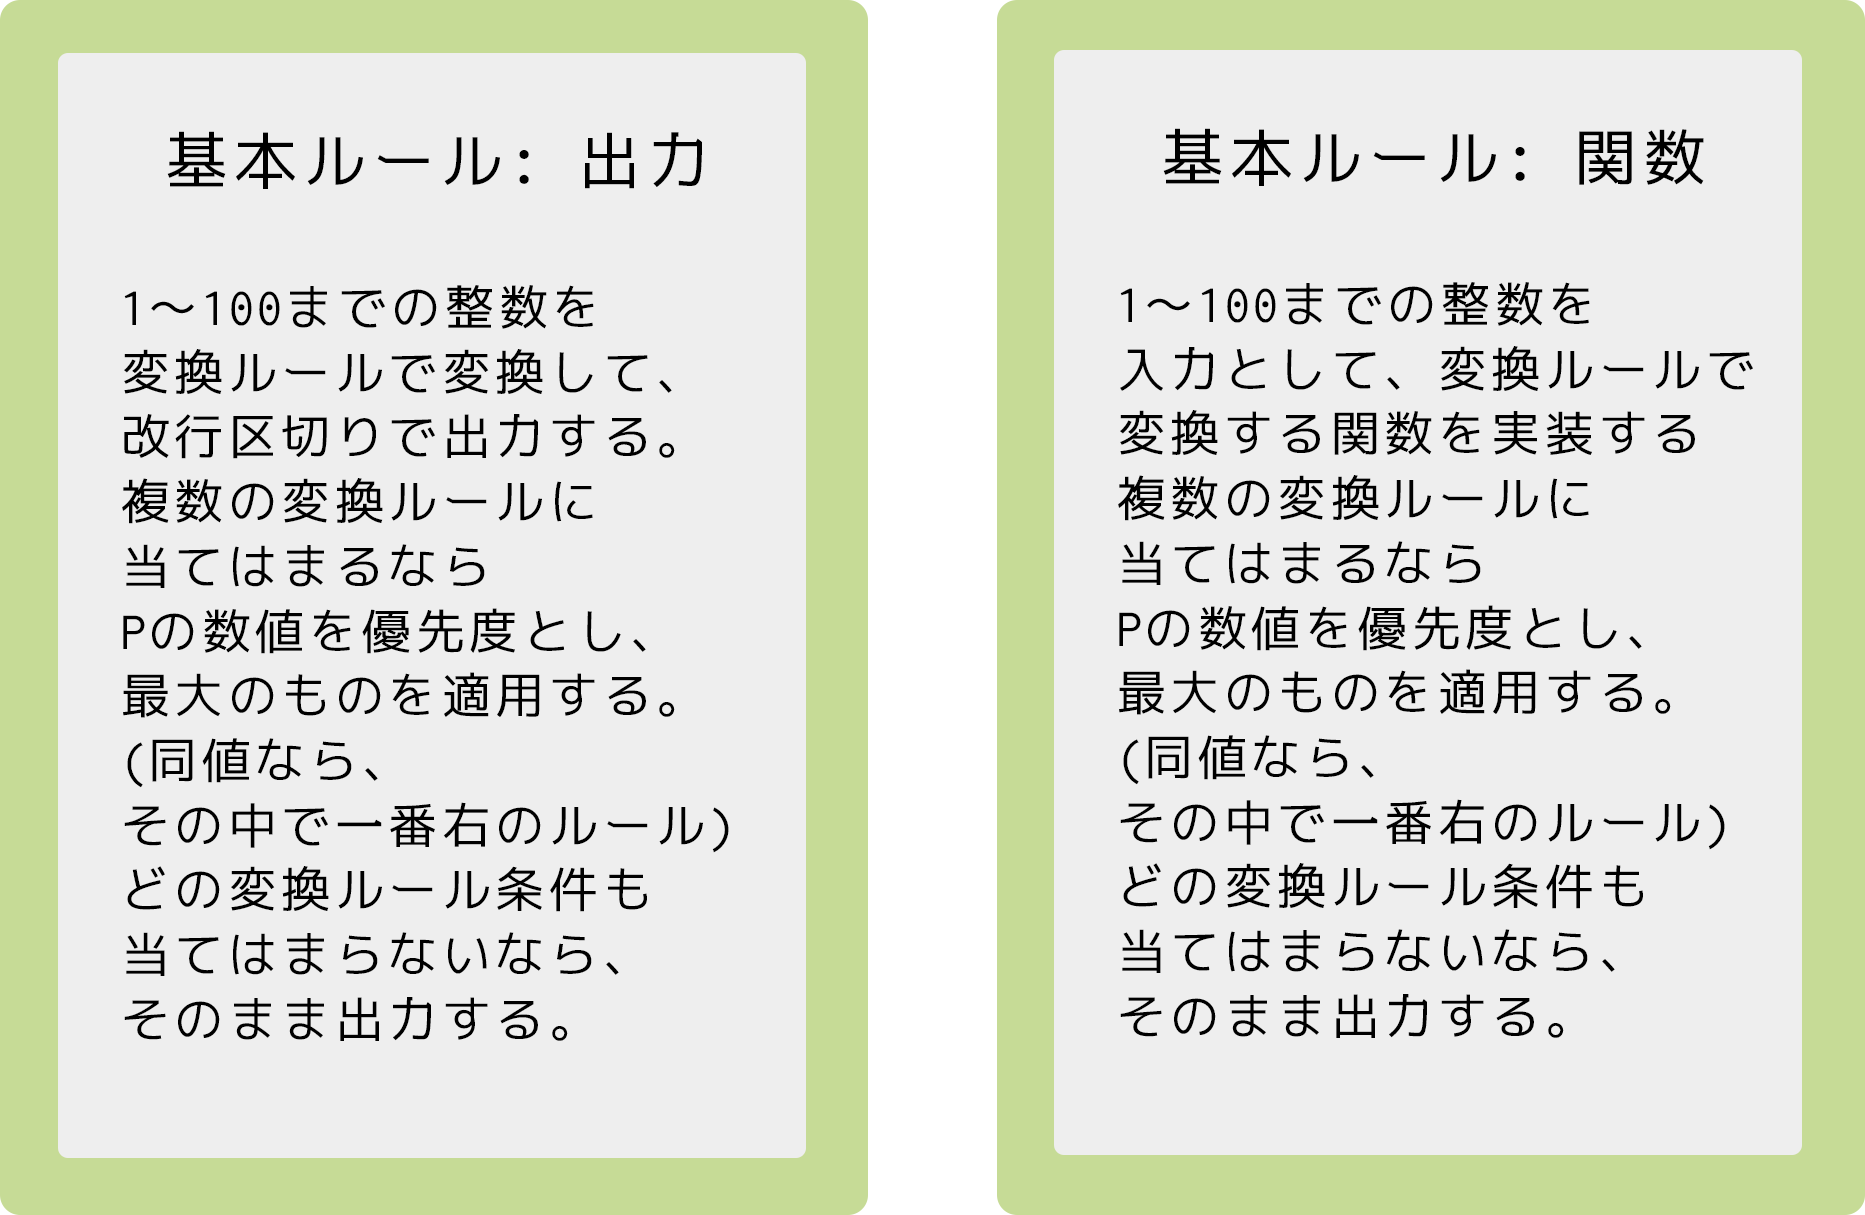
\includegraphics[height=5cm]{image/101_basic_rule_card.png}
\end{center}

{\sf 基本ルールカード}は、その名前の通りゲームの基本ルールを規定するカードです。

「基本ルール: 出力」と「基本ルール: 関数」の2種類があります。実際には、この2つは表裏に印刷され1枚のカードになっています。

  \subsection{仕様カード}
  \label{subsec:spec_card}

\begin{center}
  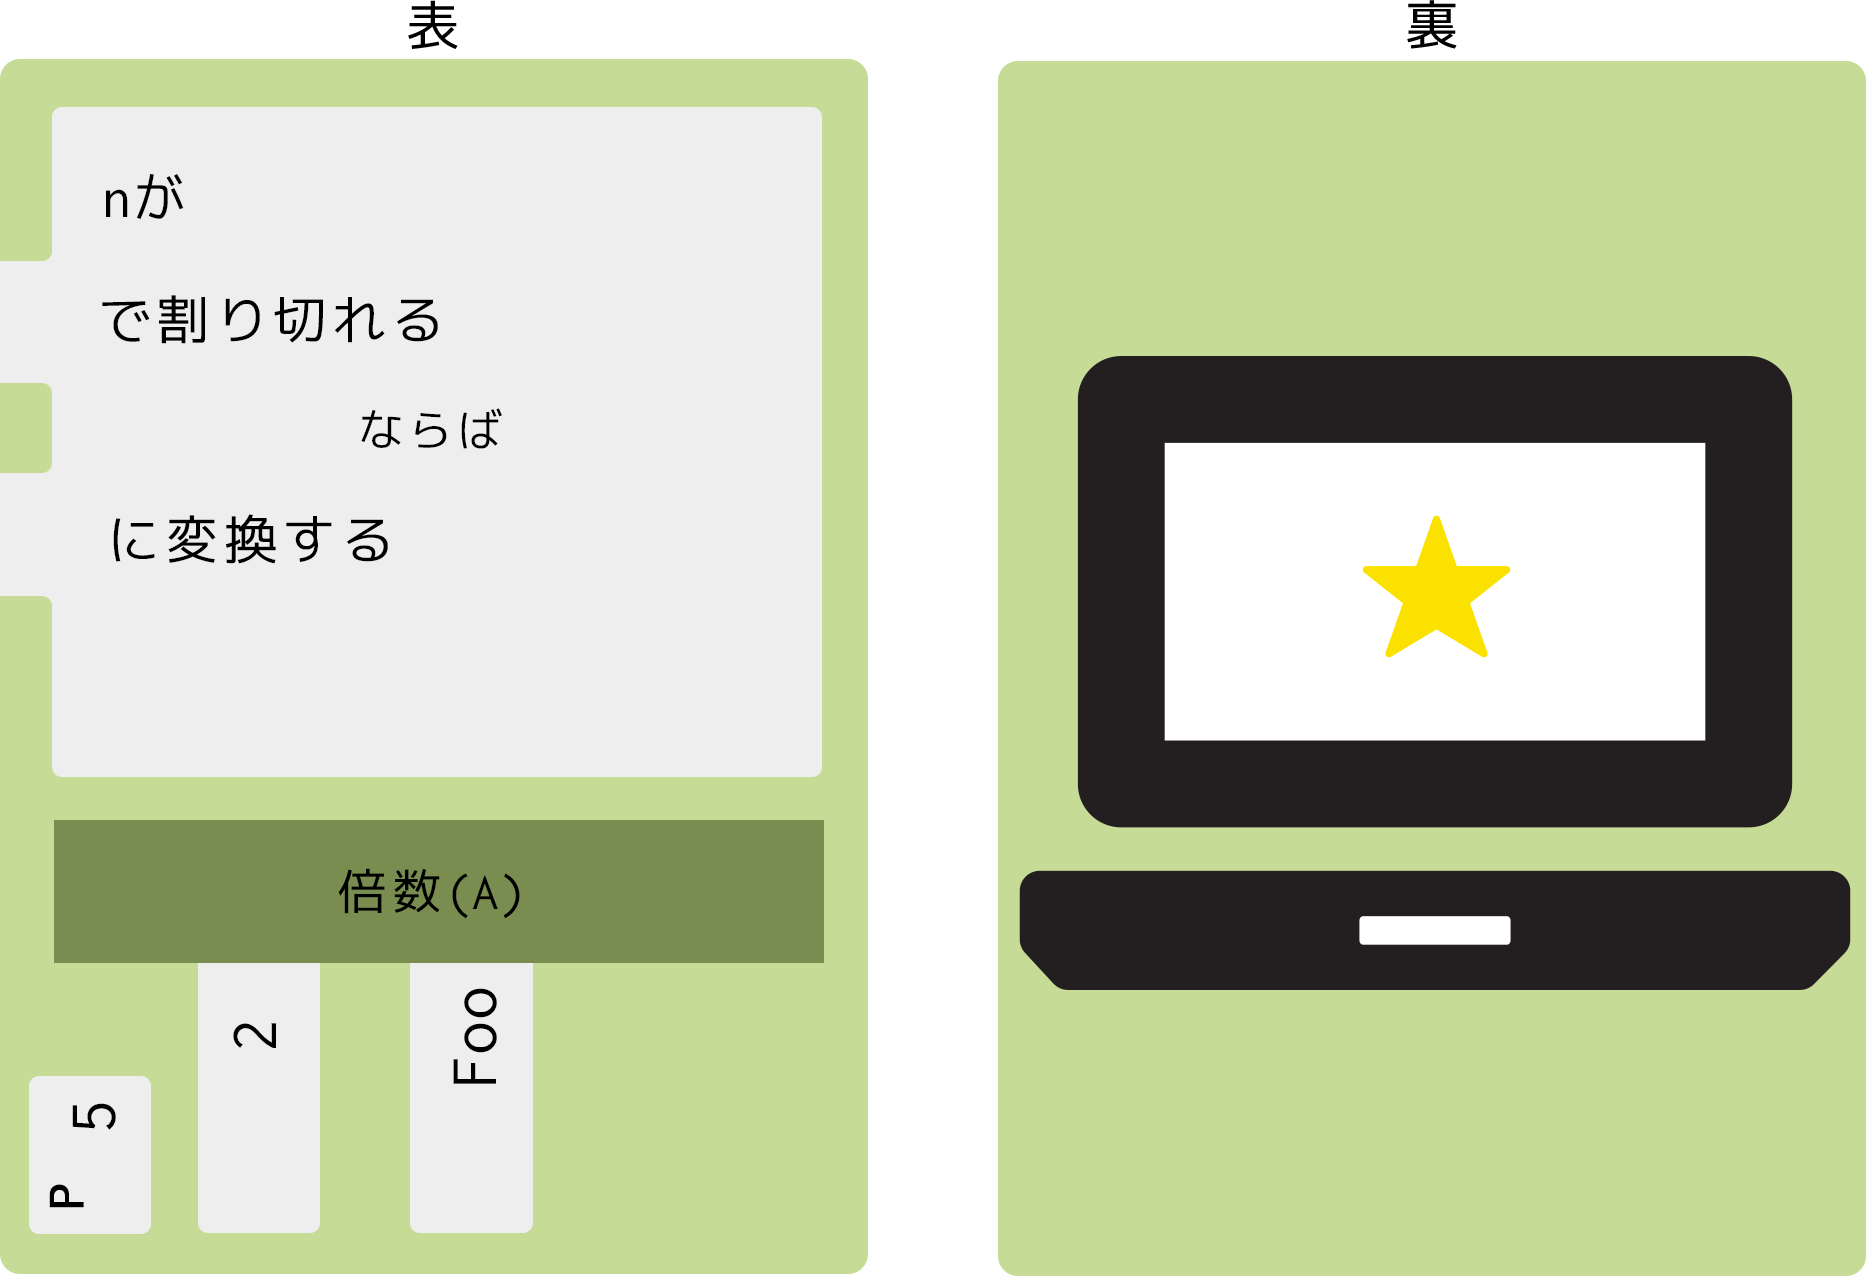
\includegraphics[height=5cm]{image/102_spec_card.png}
\end{center}

{\sf 仕様カード}は、上記のように裏面に★が書かれたカードです。

「倍数(A)」と書かれた部分が{\sf カード名}、その上が{\sf ルール文面}となっています。

下に書かれた横向きの部分は{\sf 指標}と呼びます。これはそのままでは意味を持ちません。

  \subsubsection{指標カードと変換ルール}

ゲーム中は、以下のように仕様カードの下にもう一枚の仕様カードを90°回転させて配置します。

\begin{center}
  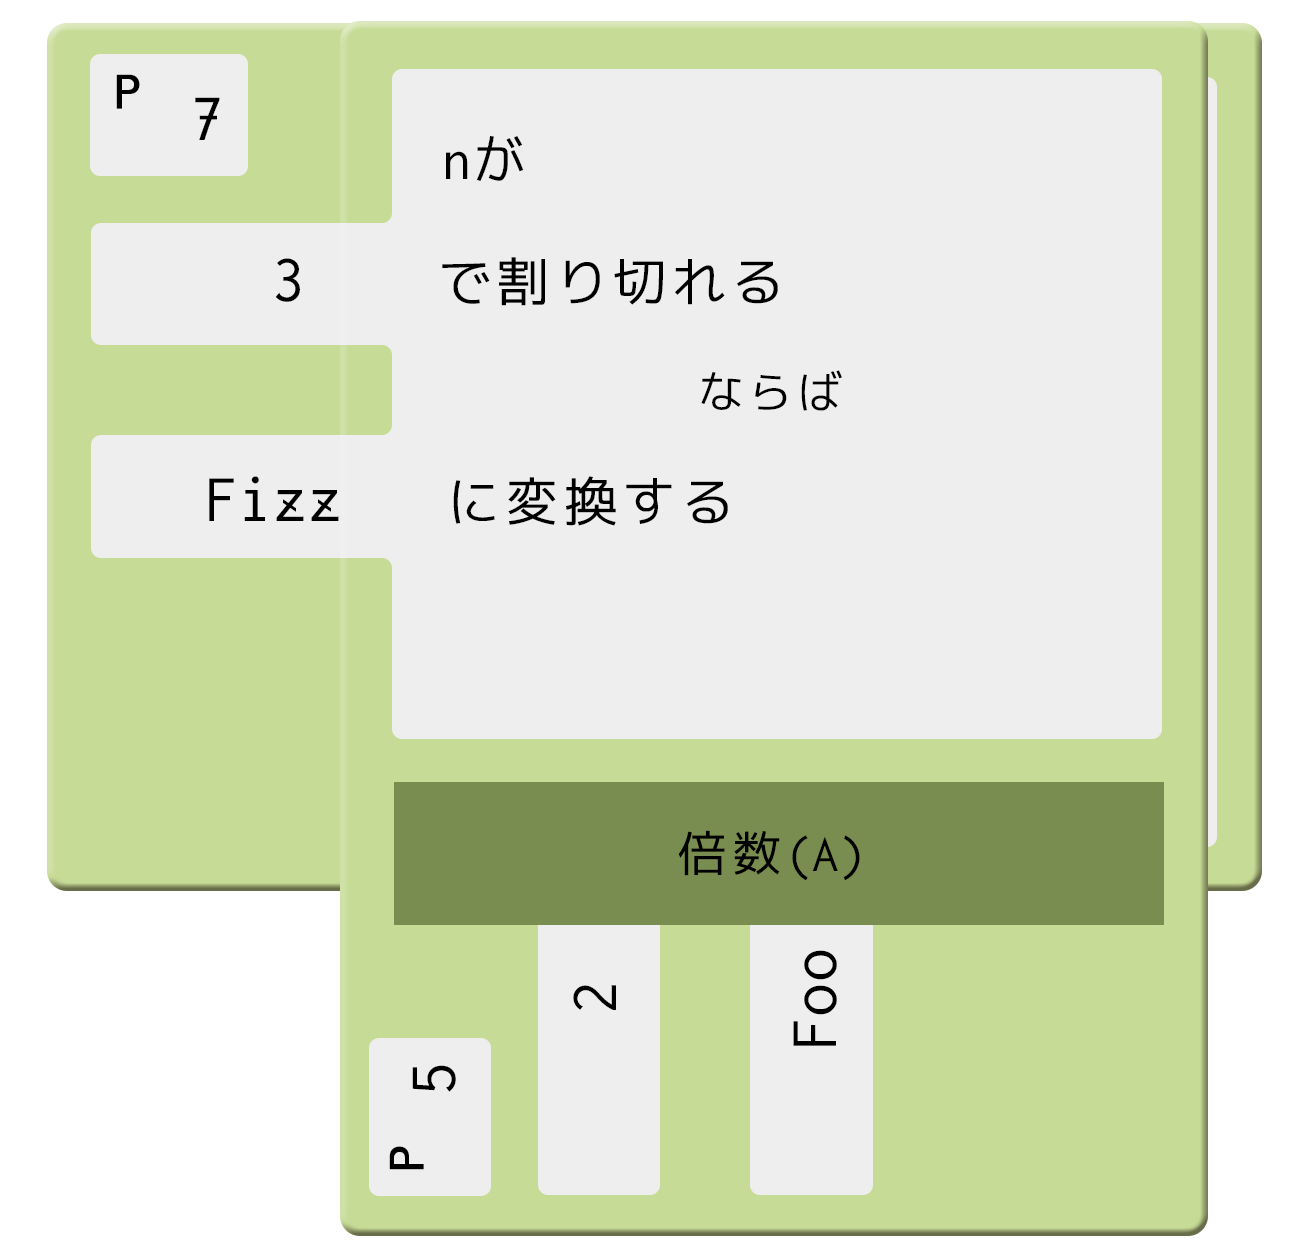
\includegraphics[height=5cm]{image/103_index_card.png}
\end{center}

このとき、下側の仕様カードを{\sf 指標カード}と呼びます。

指標カードに書かれた{\sf 指標}と、仕様カードの{\sf ルール文面}とが繋がることで1つの変換ルールを作ります。上記の例であれば、枠が繋がっているところを繋げて読み、以下のようになります。

\begin{quote}
nが
3で割り切れる
    ならば
Fizzに変換する
\end{quote}

また、左上に書かれた数値は、基本ルールで{\sf Pの数値}として参照される値です。この例では7になります。

基本的にはPの数値が大きい変換ルールほど、他のルールより優先度が高くなります。

  \subsubsection{仕様カードの難易度}

仕様カードは、裏面にかかれた★の数で1から3までの難易度に分かれています。基本的なゲームでは、それぞれの難易度ごとに山札を作ってください。

\begin{center}
  
\includegraphics[height=5cm]{image/104_spec_card_behind.png}
\end{center}

  \subsection{Rule Changeカード}
  \label{subsec:rule_change_card}

\begin{center}
  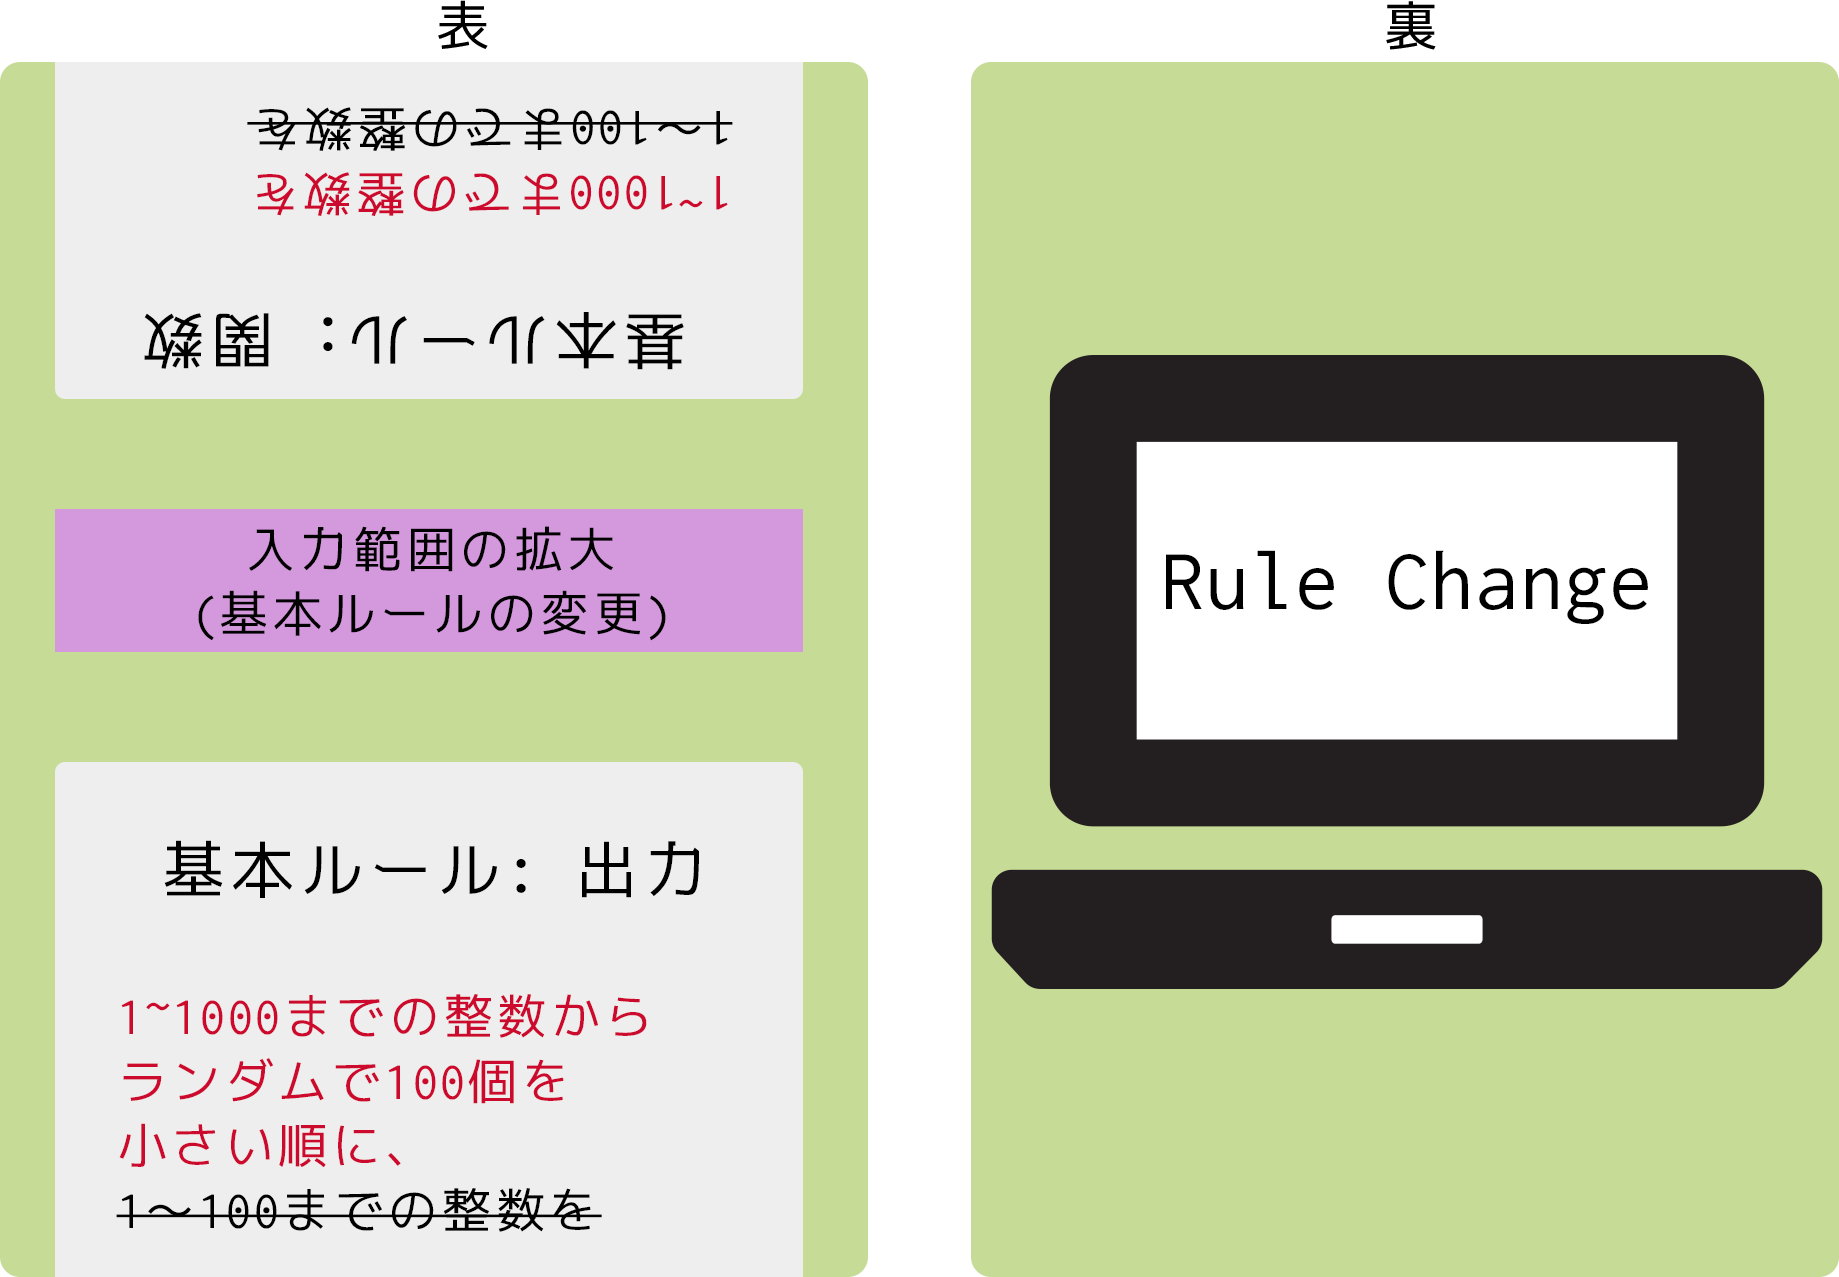
\includegraphics[height=5cm]{image/105_rule_change_card.png}
\end{center}

{\sf Rule Changeカード}は、上記のように裏面にRule Changeと書かれたカードです。

このカードには、{\sf 基本ルールの変更} と{\sf 仕様の変更}の2種類があります。

  \subsubsection{基本ルールの変更}

{\sf 基本ルールの変更}と書かれたカードには、基本ルールの一部が打ち消し線で消されて、赤字で訂正された文章が書かれています。

これらは文章が繋がるよう、基本ルールに重ねて場に出します。このとき、「入力範囲の拡大」カードのみ上に繋がるように、それ以外のカードは下に繋がるようにします。

\begin{center}
  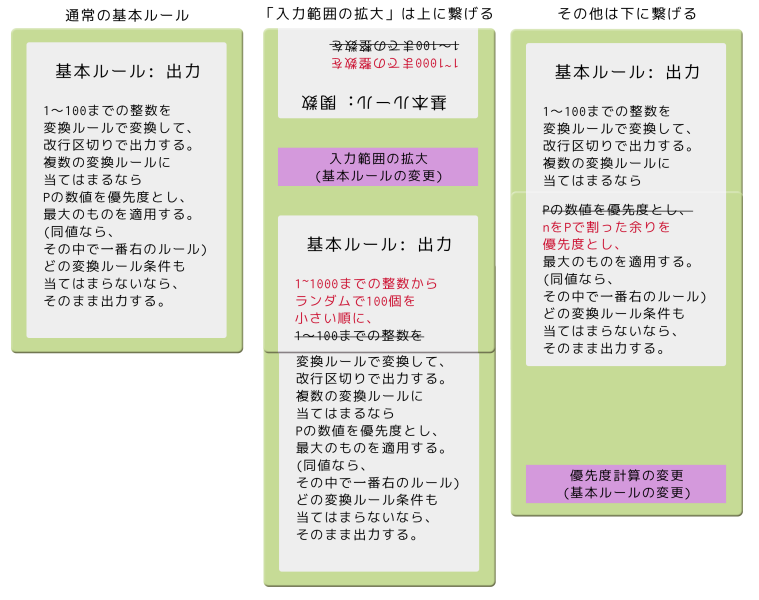
\includegraphics[height=7cm]{image/106_rule_change_apply.png}
\end{center}

これにより訂正された文章が、新しい基本ルールになります。

  \subsubsection{仕様の変更}

\begin{center}
  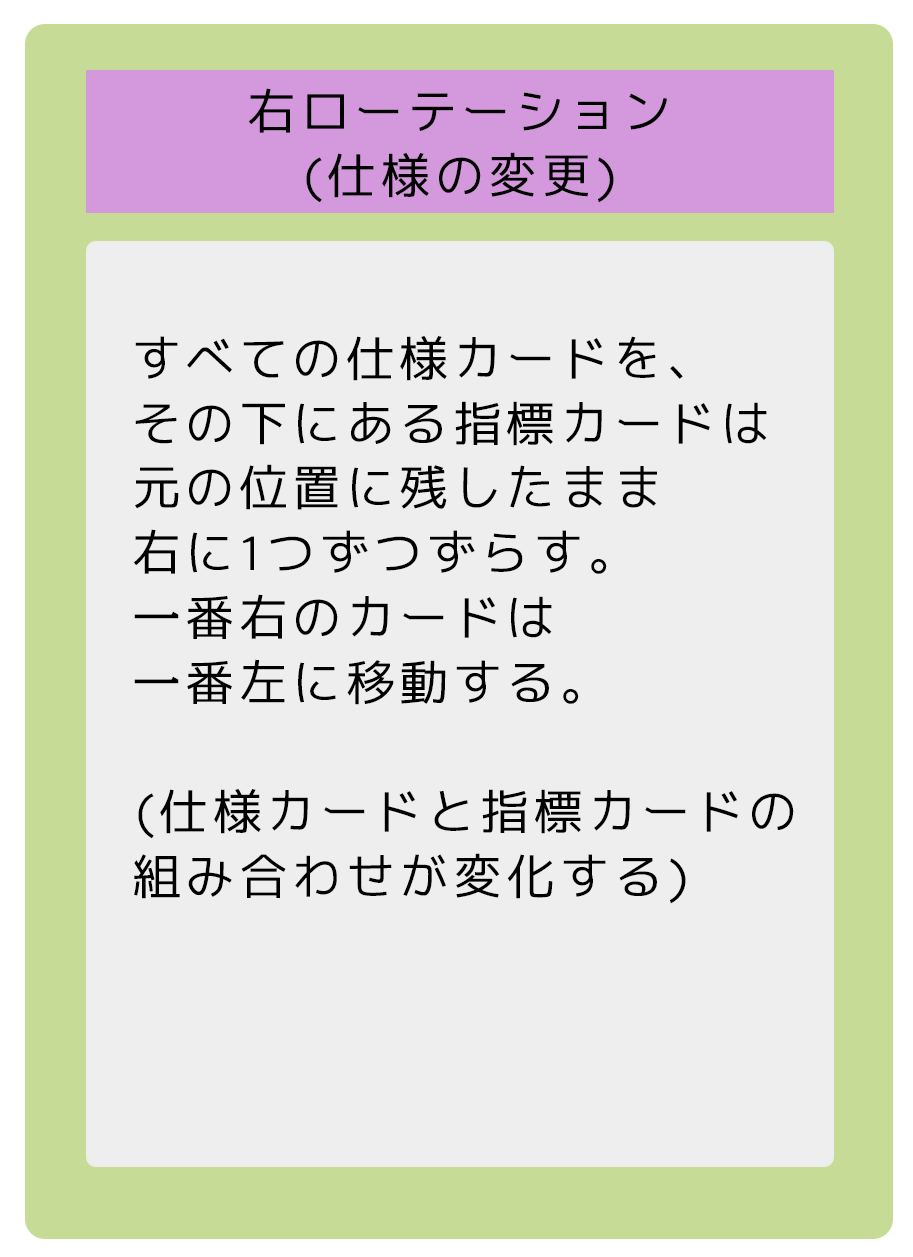
\includegraphics[height=5cm]{image/107_spec_change.png}
\end{center}

{\sf 仕様の変更}と書かれたカードには、仕様カードと指標カードに対する操作が書かれています。ゲーム時は、この手順に従って処理を行ってください。
  
  \subsection{Themeカード}

\begin{center}
  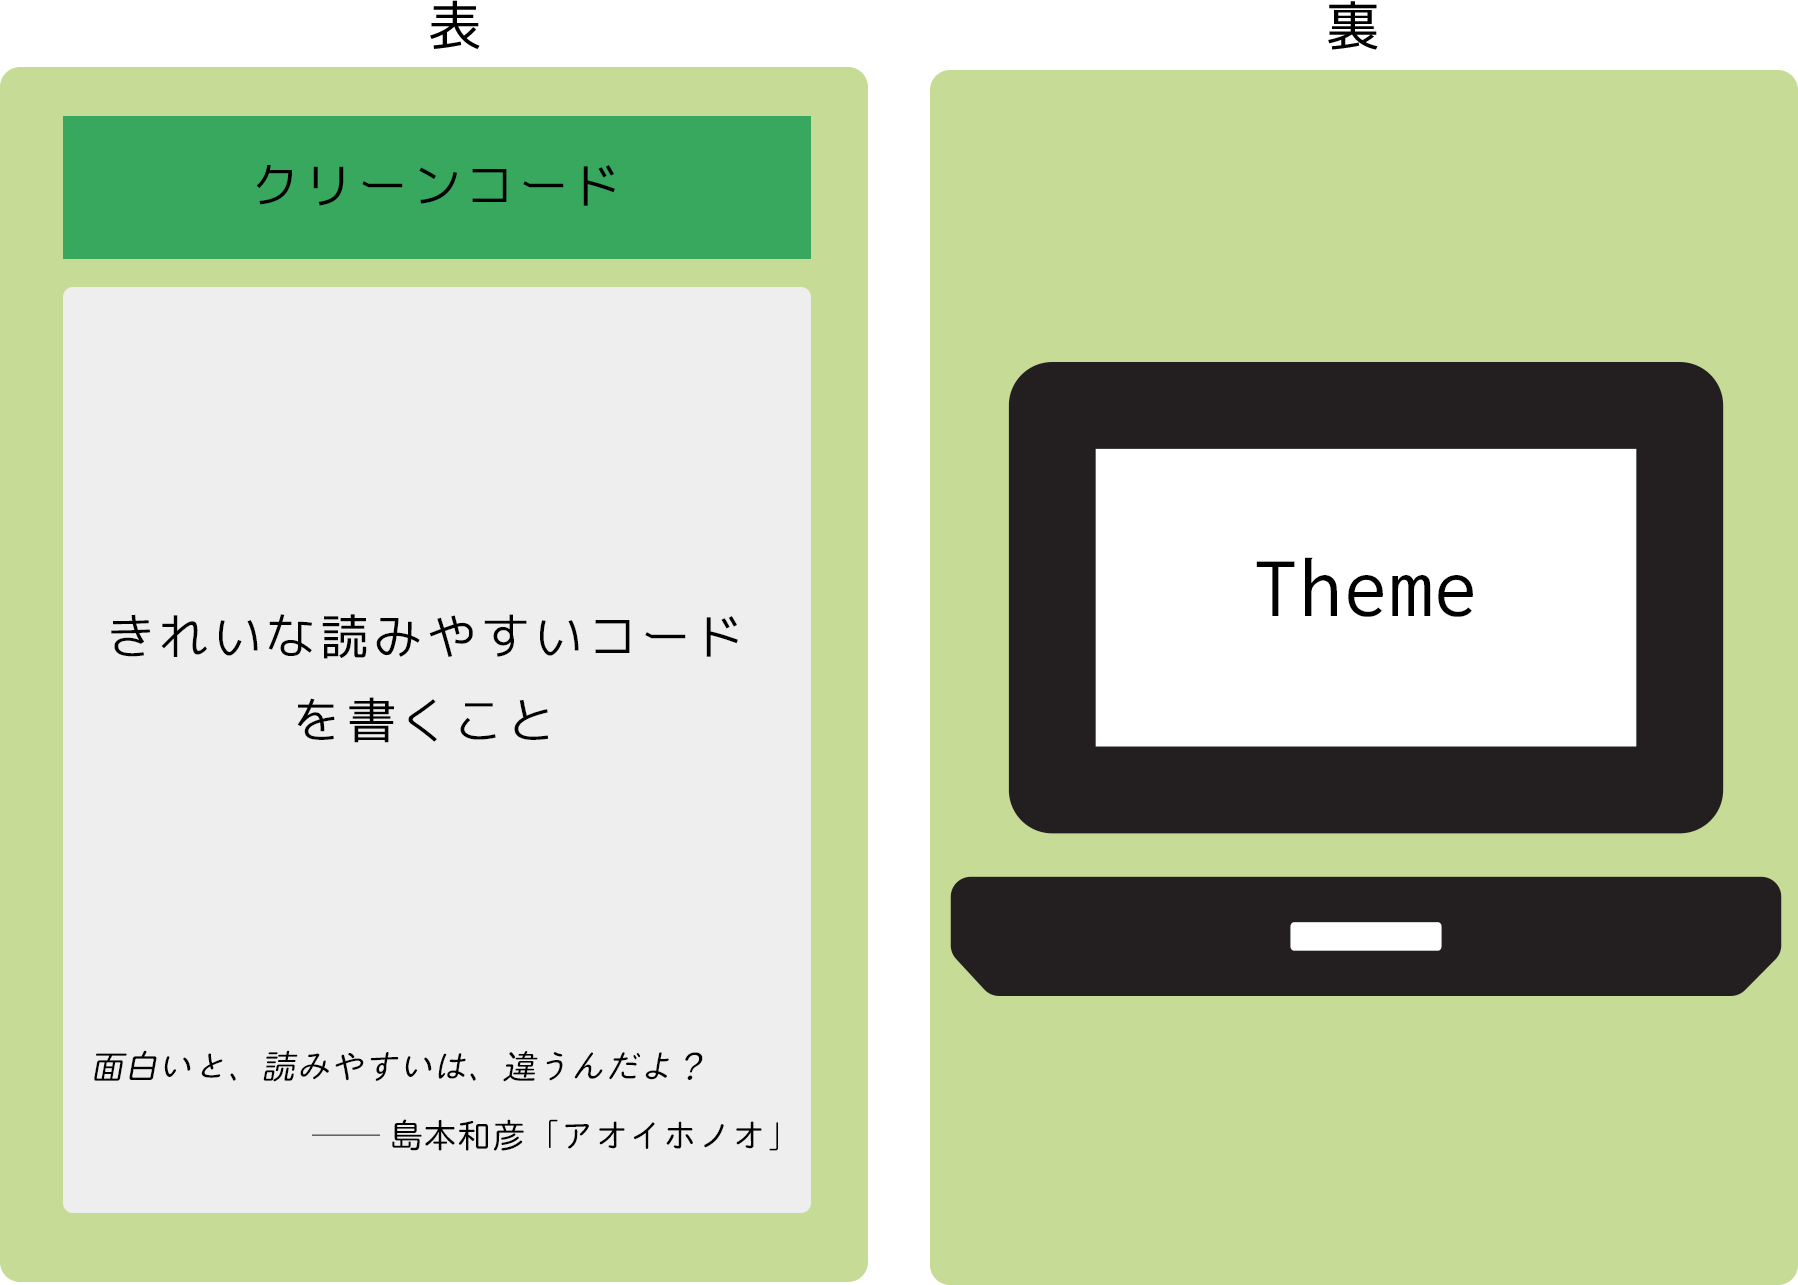
\includegraphics[height=5cm]{image/108_theme_card.png}
\end{center}

Themeカードは、上記のように裏面にThemeと書かれたカードです。このカードにはゲーム中に書くプログラムのテーマが書かれています。

なお、下部に書かれた文章はフレーバーテキストです。ゲーム上の意味はありません。

  \section{基本のゲームの流れ}
  \label{sec:game_flow}

  Programming Partyにはいくつかの遊び方がありますが、ここでは基本のゲームを取り上げてゲームの流れを紹介します。
  
  \subsection{ゲームの準備}

\begin{enumerate}
\item 「基本ルール: 出力」と「基本ルール: 関数」のいずれかを選び、全員から見やすい場所に置きます
\item 裏面のデザインごとにカードを分類し、それぞれ山にします
\item Themeの山から1枚を抜き出し、有効なテーマとして全員の見やすい場所に置きます
  \begin{itemize}
  \item 初めてのゲームでは「クリーンコード」と書かれたカードを推奨します
  \item 「エソテリック」は難易度が高いため、通常は選ばないことを推奨します
  \item 残りのThemeカードはゲームに使用しないため、箱にしまって構いません
  \end{itemize}
\item 以下の順に1枚ずつ、有効なルールとして山からカードを取って並べます
\end{enumerate}
\begin{quote}
★,★,★★,Rule Change,★★★
\end{quote}

下図のような状態になっていれば準備は完了です。

\begin{center}
  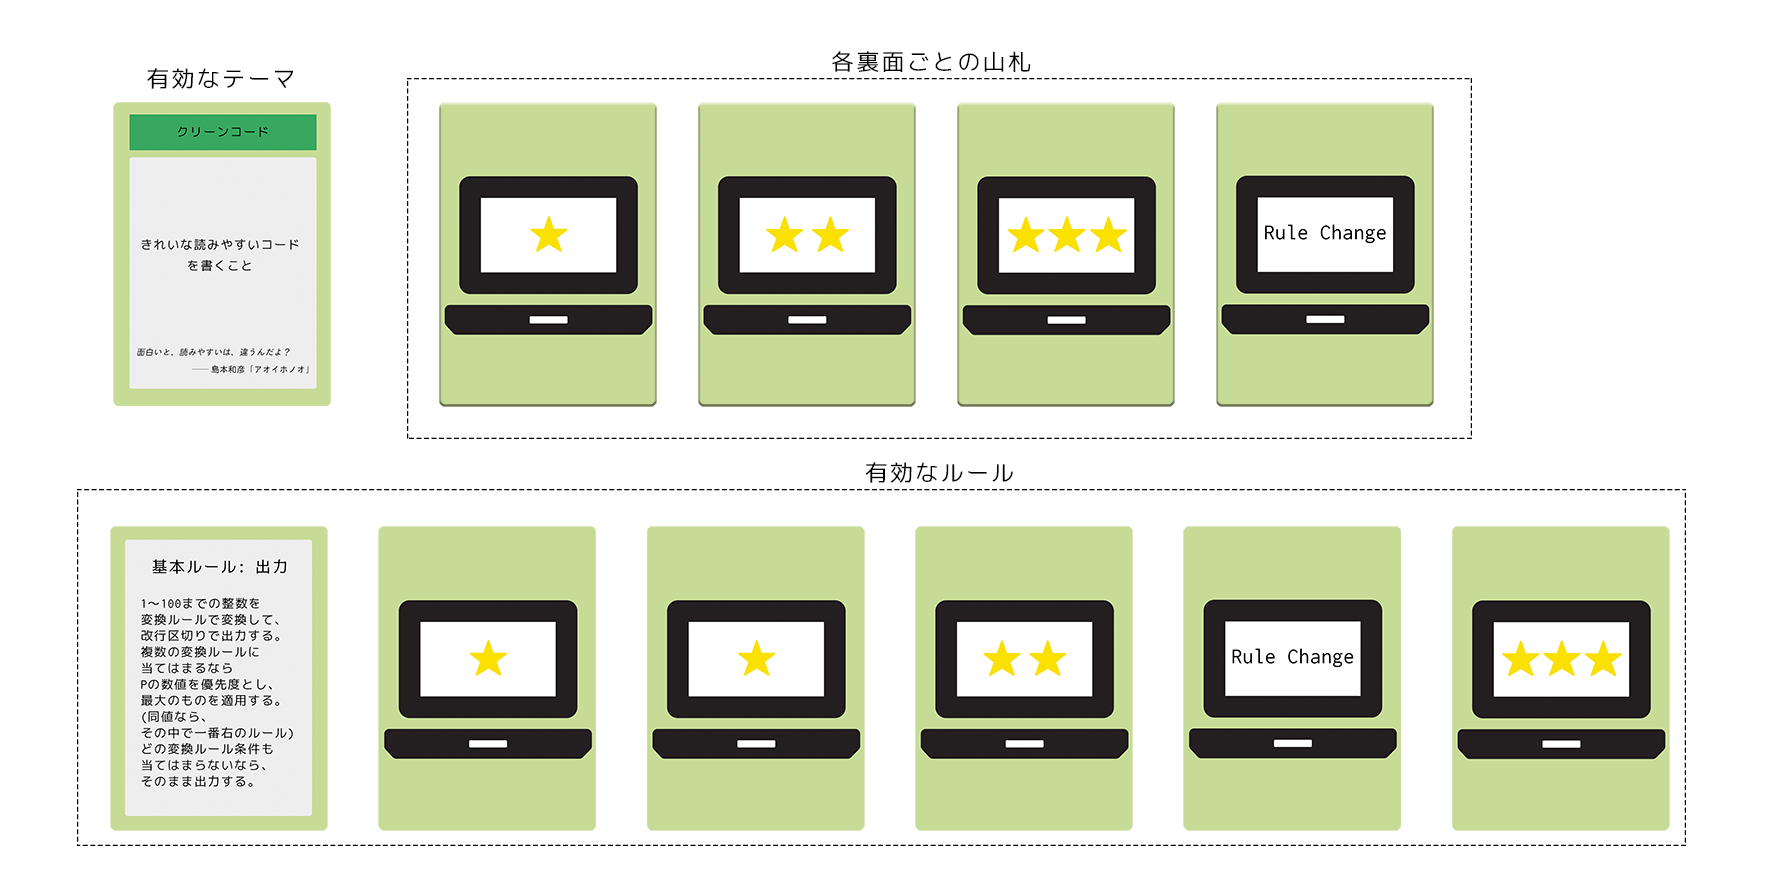
\includegraphics[height=7cm]{image/109_game_start.png}
\end{center}

  \subsection{ラウンドの流れ}

ゲームはラウンドを繰り返して進行します。1つのラウンドは以下のフェイズで構成されます。

\begin{enumerate}
\item ルールの公開
\item プログラミング
\item レビュー
\item 投票
\end{enumerate}

  \subsubsection{ルールの公開}
  
{\sf ルールの公開フェイズ}では、有効なルールにあるカードのうち、一番左にある裏向きのカードを表にします。つまり最初のラウンドでは、一番左の★カードを表にすることになります。

このとき「仕様カード」を表にした場合は、同じ★の数の山札から1枚カードを取り、指標カードとして枠が繋がるよう下に重ねます。詳しい重ね方については\ref{subsec:spec_card}節を参照してください。

また「基本ルールの変更カード」を表にした場合は、基本ルールカードと繋がるように重ねます。詳しい重ね方については\ref{subsec:rule_change_card}節を参照してください。

「仕様の変更カード」を表にした場合は、それに沿って仕様カードを動かします。

  \subsubsection{プログラミング} 

{\sf プログラミング}フェイズでは、現在有効なルールに沿って各自がプログラミングします。この際、前のラウンドまでに書いていたコードを書き換えても、新規に全てを書いても構いません。

なお、利用するプログラミング言語をどうするかや、時間制限を設けるかについてはゲーム前に確認しておくと良いでしょう。

全員がプログラムを書き終えたらプログラミングフェイズは終了です。

  \subsubsection{レビュー}

{\sf レビューフェイズ}では、お互いのコードを見せあい相互レビューを行います。

プレイヤーは任意の順に1人ずつ、自分の書いたコードを全員に見せてコードの説明をします。この際、他のプレイヤーは「仕様に沿っていない」などの間違いがあれば、それを指摘しても構いません。

全員のレビューが終わったらレビューフェイズは終了です。レビュー中に他のプレイヤーから間違いを指摘されなかったプレイヤーは、それぞれ1勝利点を獲得します。

  \subsubsection{投票} 
  
{\sf 投票フェイズ}では、テーマに沿ったと思うプレイヤーへ相互投票を行います。

各プレイヤーはレビューフェイズを踏まえ、「もっともテーマに沿ったプログラムを書いたプレイヤー」を自分以外からそれぞれ決めます。この際、多少の雑談は構いませんがそれぞれが誰にしたかは秘密裏に決定してください。

全員が決め終わったのを確認したら、合図を出して一斉にそのプレイヤーを指差してください。各プレイヤーは、これによって「自分が指差された数」だけそれぞれ勝利点を獲得します。

これで投票フェイズは終了です。また投票フェイズはラウンドの最後になるため、再度「ルールの公開」から順にラウンドを繰り返します。
 
  \subsection{ゲームの終了}

裏向きのカードを全て表にした状態でラウンドが終了したら、ゲームの終了です。基本的なルールでは、5ラウンドでゲームが終了することになります。

ゲーム終了時点で最も勝利点を獲得していたプレイヤーがゲームに勝利します。

  \section{その他のゲーム}
  \label{sec:game_online_manual}
  
基本のゲームの他に、以下のゲームモードがあります。

\begin{enumerate}
\item テスト駆動ゲーム(非対称情報での多人数対戦プレイ)
\item 協力ゲーム(非対称情報での協力プレイ)
\item ソロプレイ
\end{enumerate}

また、難易度を調整するバリアントルールもいくつか存在します。これらの情報についてはオンラインマニュアルを参照してください。\footnote[1]{ \url{ https://www.kokuyouwind.com/programming_party }}

\end{document}
